%\VignetteIndexEntry{Detecting allele-specific events from ChIP-seq data}
%\VignettePackage{BaalChIP}
%\VignetteEngine{utils::Sweave}

\documentclass{article}\usepackage[]{graphicx}\usepackage[usenames,dvipsnames]{color}
%% maxwidth is the original width if it is less than linewidth
%% otherwise use linewidth (to make sure the graphics do not exceed the margin)
\makeatletter
\def\maxwidth{ %
  \ifdim\Gin@nat@width>\linewidth
    \linewidth
  \else
    \Gin@nat@width
  \fi
}
\makeatother

\definecolor{fgcolor}{rgb}{0.345, 0.345, 0.345}
\newcommand{\hlnum}[1]{\textcolor[rgb]{0.686,0.059,0.569}{#1}}%
\newcommand{\hlstr}[1]{\textcolor[rgb]{0.192,0.494,0.8}{#1}}%
\newcommand{\hlcom}[1]{\textcolor[rgb]{0.678,0.584,0.686}{\textit{#1}}}%
\newcommand{\hlopt}[1]{\textcolor[rgb]{0,0,0}{#1}}%
\newcommand{\hlstd}[1]{\textcolor[rgb]{0.345,0.345,0.345}{#1}}%
\newcommand{\hlkwa}[1]{\textcolor[rgb]{0.161,0.373,0.58}{\textbf{#1}}}%
\newcommand{\hlkwb}[1]{\textcolor[rgb]{0.69,0.353,0.396}{#1}}%
\newcommand{\hlkwc}[1]{\textcolor[rgb]{0.333,0.667,0.333}{#1}}%
\newcommand{\hlkwd}[1]{\textcolor[rgb]{0.737,0.353,0.396}{\textbf{#1}}}%

\usepackage{framed}
\makeatletter
\newenvironment{kframe}{%
 \def\at@end@of@kframe{}%
 \ifinner\ifhmode%
  \def\at@end@of@kframe{\end{minipage}}%
  \begin{minipage}{\columnwidth}%
 \fi\fi%
 \def\FrameCommand##1{\hskip\@totalleftmargin \hskip-\fboxsep
 \colorbox{shadecolor}{##1}\hskip-\fboxsep
     % There is no \\@totalrightmargin, so:
     \hskip-\linewidth \hskip-\@totalleftmargin \hskip\columnwidth}%
 \MakeFramed {\advance\hsize-\width
   \@totalleftmargin\z@ \linewidth\hsize
   \@setminipage}}%
 {\par\unskip\endMakeFramed%
 \at@end@of@kframe}
\makeatother

\definecolor{shadecolor}{rgb}{.97, .97, .97}
\definecolor{messagecolor}{rgb}{0, 0, 0}
\definecolor{warningcolor}{rgb}{1, 0, 1}
\definecolor{errorcolor}{rgb}{1, 0, 0}
\newenvironment{knitrout}{}{} % an empty environment to be redefined in TeX

\usepackage{alltt}

\RequirePackage{/Library/Frameworks/R.framework/Versions/3.1/Resources/library/BiocStyle/resources/latex/Bioconductor}

\AtBeginDocument{\bibliographystyle{/Library/Frameworks/R.framework/Versions/3.1/Resources/library/BiocStyle/resources/latex/unsrturl}}


\IfFileExists{upquote.sty}{\usepackage{upquote}}{}
\begin{document}




\title{Detecting allele-specific events from ChIP-seq data}
\author{Ines de Santiago, Wei Liu, Ke Yuan, Florian Markowetz}

\date{Edited: 2015; Compiled: \today}

\maketitle

\tableofcontents

\section{Introduction}

Allele-specific binding (ASB) measurements of transcription-factor binding from ChIP-seq data have provided important insights into the allelic effects of non-coding variants and its contribution to phenotypic diversity. However, such approaches are designed to examine the allelic imbalances in diploid samples and do not address copy number differences between the two alleles, a known phenotypical feature of cancer cells.

BaalChIP (Baysian Anaysis of Allelic imbalances from ChIP-seq data) tests the differential read counts of the alleles at each heterozygous variant using the quantitative information of ChIP-seq read counts at the reference and alternative alleles and accomodating the information about the allele presence and other sources of ChIP-seq mapping biases.


\section{Example}

This section offers a quick example of how to use BaalChIP to identify ASB events with correction for relative allele frequency.

\subsection{Identifying allele-specific binding (ASB) events from ChIP-seq data obtained from cancer cells}

The example dataset contains ChIP-seq data obtained for two cell lines: A cancer cell-line (MCF7) and a normal cell line (GM12891). For each cell line, ChIP-seq data exists for four transcription factors and two biological replicates for each of the transcription factors.

The metadata and all files necessary for this example are available in the extra subdirectory
of the BaalChIP package directory; you can make this your working directory by entering:

\begin{knitrout}
\definecolor{shadecolor}{rgb}{0.969, 0.969, 0.969}\color{fgcolor}\begin{kframe}
\begin{alltt}
\hlkwd{library}\hlstd{(BaalChIP)}
\hlkwd{setwd}\hlstd{(}\hlkwd{system.file}\hlstd{(}\hlstr{"test"}\hlstd{,}\hlkwc{package}\hlstd{=}\hlstr{"BaalChIP"}\hlstd{))}
\end{alltt}
\end{kframe}
\end{knitrout}
Note that the example data in this vignette does not reveal real biology and was build only for demonstration purposes.

The first step is to contruct a BaalChIP object:
\begin{knitrout}
\definecolor{shadecolor}{rgb}{0.969, 0.969, 0.969}\color{fgcolor}\begin{kframe}
\begin{alltt}
\hlstd{samplesheet} \hlkwb{<-} \hlstr{"example.tsv"}
\hlstd{hets} \hlkwb{<-} \hlkwd{c}\hlstd{(}\hlstr{"MCF7"}\hlstd{=}\hlstr{"MCF7_hetSNP.txt"}\hlstd{,} \hlstr{"GM12891"}\hlstd{=}\hlstr{"GM12891_hetSNP.txt"}\hlstd{)}
\hlstd{res} \hlkwb{<-} \hlkwd{new}\hlstd{(}\hlstr{"BaalChIP"}\hlstd{,} \hlkwc{samplesheet}\hlstd{=samplesheet,} \hlkwc{hets}\hlstd{=hets)}
\end{alltt}
\end{kframe}
\end{knitrout}

Given a new BaalChIP object, allele-specific binding events can be identified as follows:
\begin{knitrout}
\definecolor{shadecolor}{rgb}{0.969, 0.969, 0.969}\color{fgcolor}\begin{kframe}
\begin{alltt}
\hlcom{#first load some data}
\hlkwd{data}\hlstd{(blacklist_hg19)}
\hlkwd{data}\hlstd{(pickrell2011cov1_hg19)}
\hlkwd{data}\hlstd{(UniqueMappability50bp_hg19)}

\hlcom{#run example}
\hlstd{res} \hlkwb{<-} \hlkwd{alleleCounts}\hlstd{(res,} \hlkwc{min_base_quality}\hlstd{=}\hlnum{10}\hlstd{,} \hlkwc{min_mapq}\hlstd{=}\hlnum{15}\hlstd{)}
\hlstd{res} \hlkwb{<-} \hlkwd{QCfilter}\hlstd{(res,}
                \hlkwc{RegionsToFilter}\hlstd{=}\hlkwd{list}\hlstd{(}\hlstr{"blacklist"}\hlstd{=blacklist_hg19,}
                                     \hlstr{"highcoverage"}\hlstd{=pickrell2011cov1_hg19),}
                \hlkwc{RegionsToKeep}\hlstd{=}\hlkwd{list}\hlstd{(}\hlstr{"UniqueMappability"}\hlstd{=UniqueMappability50bp_hg19))}
\hlstd{res} \hlkwb{<-} \hlkwd{mergePerGroup}\hlstd{(res)}
\hlstd{res} \hlkwb{<-} \hlkwd{filter1allele}\hlstd{(res)}
\hlstd{res} \hlkwb{<-} \hlkwd{getASB}\hlstd{(res,} \hlkwc{Iter}\hlstd{=}\hlnum{5000}\hlstd{,} \hlkwc{conf_level}\hlstd{=}\hlnum{0.95}\hlstd{)}
\end{alltt}
\end{kframe}
\end{knitrout}

If you trust the package defaults, the first four steps can be replaced by a wrapper function, making BaalChIP workflow possible to run a 3-step script:
\begin{knitrout}
\definecolor{shadecolor}{rgb}{0.969, 0.969, 0.969}\color{fgcolor}\begin{kframe}
\begin{alltt}
\hlstd{res} \hlkwb{<-} \hlkwd{new}\hlstd{(}\hlstr{"BaalChIP"}\hlstd{,} \hlkwc{samplesheet}\hlstd{=samplesheet,} \hlkwc{hets}\hlstd{=hets)}
\hlstd{res} \hlkwb{<-} \hlkwd{BaalChIP.QC}\hlstd{(res)}
\hlstd{res} \hlkwb{<-} \hlkwd{getASB}\hlstd{(res)}
\end{alltt}
\end{kframe}
\end{knitrout}

The following sections describe these steps in more detail.

\subsection{Data preparation}

In order to run BaalChIP, one needs to generate a sample sheet describing the samples and the groups within each study. This file should be saved as a tab-delimited file.
A .tsv sample sheet has been included in this vignette and can be assessed as follows:

\begin{knitrout}
\definecolor{shadecolor}{rgb}{0.969, 0.969, 0.969}\color{fgcolor}\begin{kframe}
\begin{alltt}
\hlkwd{setwd}\hlstd{(}\hlkwd{system.file}\hlstd{(}\hlstr{"test"}\hlstd{,}\hlkwc{package}\hlstd{=}\hlstr{"BaalChIP"}\hlstd{))}
\hlstd{samplesheet} \hlkwb{<-} \hlkwd{read.delim}\hlstd{(}\hlstr{"example.tsv"}\hlstd{)}
\hlstd{samplesheet}
\end{alltt}
\begin{verbatim}
##    group_name target replicate_number                       bam_name
## 1        MCF7   cFOS                1    bamFIles/MCF7_cFOS_Rep1.bam
## 2        MCF7   cFOS                2    bamFiles/MCF7_cFOS_Rep2.bam
## 3        MCF7   cMYC                1    bamFiles/MCF7_cMYC_Rep1.bam
## 4        MCF7   cMYC                2    bamFiles/MCF7_cMYC_Rep2.bam
## 5        MCF7   POL2                1    bamFiles/MCF7_POL2_Rep1.bam
## 6        MCF7   POL2                2    bamFiles/MCF7_POL2_Rep2.bam
## 7        MCF7  STAT3                1   bamFiles/MCF7_STAT3_Rep1.bam
## 8        MCF7  STAT3                2   bamFiles/MCF7_STAT3_Rep2.bam
## 9     GM12891   POL2                1 bamFiles/GM12891_POL2_Rep1.bam
## 10    GM12891   POL2                2 bamFiles/GM12891_POL2_Rep2.bam
## 11    GM12891   PAX5                1 bamFiles/GM12891_PAX5_Rep1.bam
## 12    GM12891   PAX5                2 bamFiles/GM12891_PAX5_Rep2.bam
## 13    GM12891    PU1                1  bamFiles/GM12891_PU1_Rep1.bam
## 14    GM12891    PU1                2  bamFiles/GM12891_PU1_Rep2.bam
## 15    GM12891   TAF1                1 bamFiles/GM12891_TAF1_Rep1.bam
## 16    GM12891   TAF1                2 bamFiles/GM12891_TAF1_Rep2.bam
##                     bed_name
## 1     bedFiles/MCF7_cFOS.bed
## 2     bedFiles/MCF7_cFOS.bed
## 3     bedFiles/MCF7_cMYC.bed
## 4    bedFiles//MCF7_cMYC.bed
## 5     bedFiles/MCF7_POL2.bed
## 6     bedFiles/MCF7_POL2.bed
## 7    bedFiles/MCF7_STAT3.bed
## 8    bedFiles/MCF7_STAT3.bed
## 9  bedFiles/GM12891_POL2.bed
## 10 bedFiles/GM12891_POL2.bed
## 11 bedFiles/GM12891_PAX5.bed
## 12 bedFiles/GM12891_PAX5.bed
## 13  bedFiles/GM12891_PU1.bed
## 14  bedFiles/GM12891_PU1.bed
## 15 bedFiles/GM12891_TAF1.bed
## 16 bedFiles/GM12891_TAF1.bed
\end{verbatim}
\end{kframe}
\end{knitrout}

This sample sheet details the metadata for ChIP-seq studies in MCF7 and GM12891 cell lines. For each study, ChIP-seq data exists for four transcription factors (\textt{target}). The first column \texttt{group name} identifies the group label of each study (MCF7, GM12891). The column \texttt{replicate number} shows that there are two biological replicates for each ChIP-seq factor. The sample sheet also contains file paths to the BAM files (\texttt{bam name}) with the aligned reads and the BED files (\texttt{bed name}) with the previously called peaks. 


Note that the sample sheet should be saved as a .csv file, you do not have to first load it into a data frame (the filename is passed directly to BaalChIP).

In addition to the sample sheet, BaalChIP requires a 'variant file' containning the list of heterozygous variants to be analysed. As an example, a small set of heterozygous variants for each cell line has been included in this vignette and can be assessed as follows:

\begin{knitrout}
\definecolor{shadecolor}{rgb}{0.969, 0.969, 0.969}\color{fgcolor}\begin{kframe}
\begin{alltt}
\hlkwd{head}\hlstd{(}\hlkwd{read.delim}\hlstd{(}\hlstr{"MCF7_hetSNP.txt"}\hlstd{))}
\hlkwd{head}\hlstd{(}\hlkwd{read.delim}\hlstd{(}\hlstr{"GM12891_hetSNP.txt"}\hlstd{))}
\end{alltt}
\end{kframe}
\end{knitrout}

The information in the variant file should include an \textt{ID} column with a unique identifier string per variant, the (1-based) genomic coordinates \textt{CHROM, POS}, and the A,C,G,T bases for the reference \textt{REF} and the non-reference alternate \textt{ALT} allele. The final column \textt{RAF} consists of a 
value ranging from 0 to 1 for each variant denoting the relative allele frequency. A value between 0.5 and 1 denotes a bias to the reference allele, and a value between 0 and 0.5 a bias to the alternate allele. This column is optional, if missing BaalChIP will still run but will not correct for relative allele frequency (copy-number) bias.


\subsection{Constructing a BaalChIP object}

The first step is to generate a BaalChIP object. The function \textt{new} accepts a samplesheet and a named vector containing the filenames for the variant files to be used. The names in the vector should correspond to \textt{group_name} strings in the \textt{.csv} samplesheet, in this case it should be "MCF7" and "GM12891".

\begin{knitrout}
\definecolor{shadecolor}{rgb}{0.969, 0.969, 0.969}\color{fgcolor}\begin{kframe}
\begin{alltt}
\hlstd{samplesheet} \hlkwb{<-} \hlstr{"example.tsv"}
\hlstd{hets} \hlkwb{<-} \hlkwd{c}\hlstd{(}\hlstr{"MCF7"}\hlstd{=}\hlstr{"MCF7_hetSNP.txt"}\hlstd{,} \hlstr{"GM12891"}\hlstd{=}\hlstr{"GM12891_hetSNP.txt"}\hlstd{)}
\hlstd{res} \hlkwb{<-} \hlkwd{new}\hlstd{(}\hlstr{"BaalChIP"}\hlstd{,} \hlkwc{samplesheet}\hlstd{=samplesheet,} \hlkwc{hets}\hlstd{=hets)}
\end{alltt}
\end{kframe}
\end{knitrout}

the samplesheet is saved in the \textt{samples} slot of a BaalChIP object:

\begin{knitrout}
\definecolor{shadecolor}{rgb}{0.969, 0.969, 0.969}\color{fgcolor}\begin{kframe}
\begin{alltt}
\hlstd{res}\hlopt{@}\hlkwc{samples}
\end{alltt}
\end{kframe}
\end{knitrout}

\subsection{Obtainning allele-specific counts for BAM files}

The next step is to compute the read coverage at each allele. BaalChIP will read in the information whithin the \textt{samples} slot of a BaalChIP object and it will primarly find all variants overlapping peaks. Then, for each variant, computes the number of reads carrying the reference (REF) and alternative (ALT) alleles.

\begin{knitrout}
\definecolor{shadecolor}{rgb}{0.969, 0.969, 0.969}\color{fgcolor}\begin{kframe}
\begin{alltt}
\hlstd{res} \hlkwb{<-} \hlkwd{alleleCounts}\hlstd{(res,} \hlkwc{min_base_quality}\hlstd{=}\hlnum{10}\hlstd{,} \hlkwc{min_mapq}\hlstd{=}\hlnum{15}\hlstd{)}
\hlstd{res}
\end{alltt}
\end{kframe}
\end{knitrout}

\subsection{QC: Filtering variants that may be problematic for allele-specific detection}

BaalChIP contains an extensive set of filters...

\begin{knitrout}
\definecolor{shadecolor}{rgb}{0.969, 0.969, 0.969}\color{fgcolor}\begin{kframe}
\begin{alltt}
\hlstd{res} \hlkwb{<-} \hlkwd{QCfilter}\hlstd{(res,}
                \hlkwc{RegionsToFilter}\hlstd{=}\hlkwd{list}\hlstd{(}\hlstr{"blacklist"}\hlstd{=blacklist_hg19,} \hlstr{"highcoverage"}\hlstd{=pickrell2011cov1_hg19),}
                \hlkwc{RegionsToKeep}\hlstd{=}\hlkwd{list}\hlstd{(}\hlstr{"UniqueMappability"}\hlstd{=UniqueMappability50bp_hg19))}
\hlstd{res} \hlkwb{<-} \hlkwd{mergePerGroup}\hlstd{(res)}
\hlstd{res} \hlkwb{<-} \hlkwd{filter1allele}\hlstd{(res)}
\end{alltt}
\end{kframe}
\end{knitrout}

\subsection{Allele counts and QC in 1-step script}

\begin{knitrout}
\definecolor{shadecolor}{rgb}{0.969, 0.969, 0.969}\color{fgcolor}\begin{kframe}
\begin{alltt}
\hlstd{res} \hlkwb{<-} \hlkwd{new}\hlstd{(}\hlstr{"BaalChIP"}\hlstd{, samplesheet, hets)}
\hlstd{res} \hlkwb{<-} \hlkwd{BaalChIP.QC}\hlstd{(res)}
\end{alltt}
\end{kframe}
\end{knitrout}

\subsection{summarysing and plotting QC data}



\begin{knitrout}
\definecolor{shadecolor}{rgb}{0.969, 0.969, 0.969}\color{fgcolor}\begin{kframe}
\begin{alltt}
\hlkwd{data}\hlstd{(baalObject)}
\hlkwd{plotQC}\hlstd{(res,} \hlstr{"barplot_per_group"}\hlstd{)}
\end{alltt}
\end{kframe}

{\centering 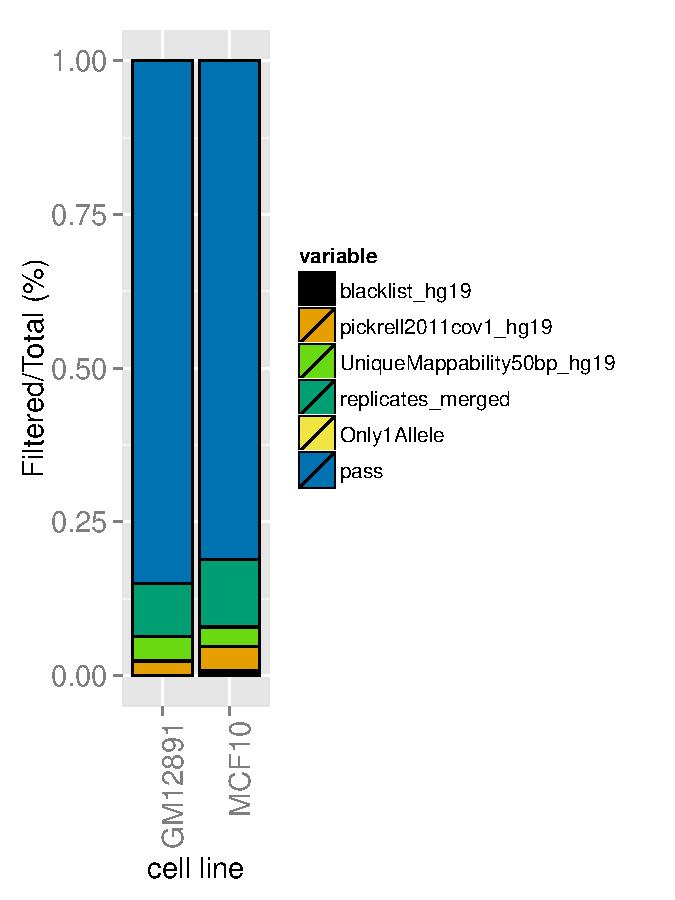
\includegraphics[width=\maxwidth]{figure/QCplots-1} 

}


\begin{kframe}\begin{alltt}
\hlkwd{plotQC}\hlstd{(res,} \hlstr{"boxplot_per_filter"}\hlstd{)}
\end{alltt}
\end{kframe}

{\centering 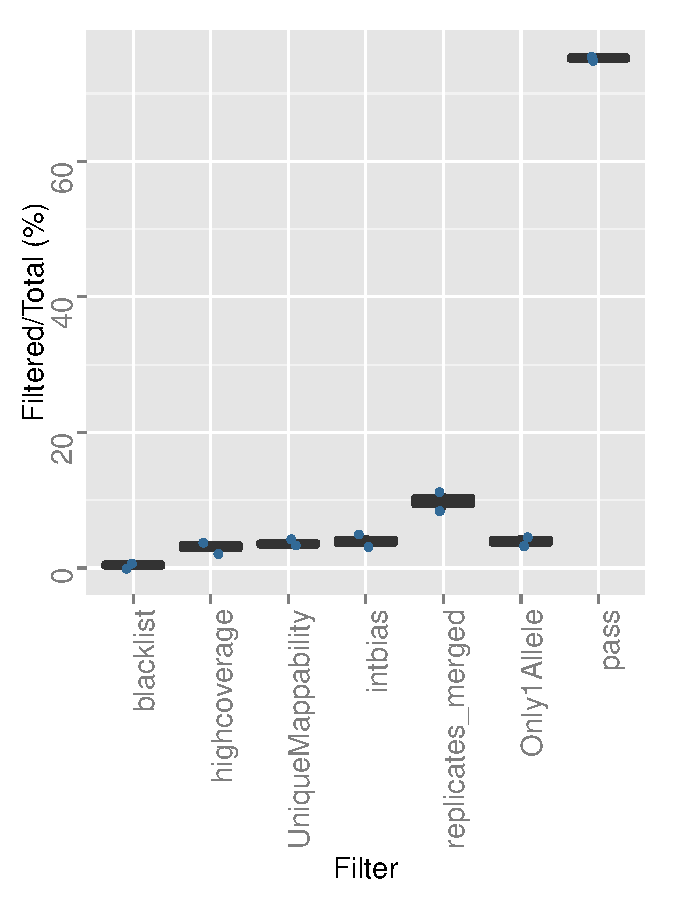
\includegraphics[width=\maxwidth]{figure/QCplots-2} 

}


\begin{kframe}\begin{alltt}
\hlkwd{plotQC}\hlstd{(res,} \hlstr{"overall_pie"}\hlstd{)}
\end{alltt}
\end{kframe}

{\centering 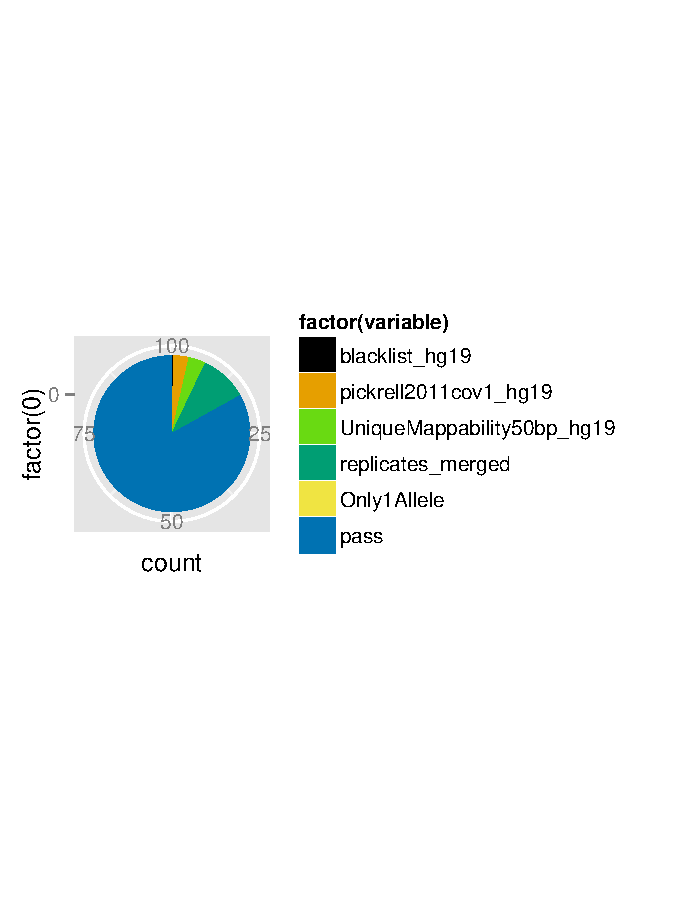
\includegraphics[width=\maxwidth]{figure/QCplots-3} 

}


\begin{kframe}\begin{alltt}
\hlkwd{summaryQC}\hlstd{(res)}
\end{alltt}
\begin{verbatim}
## $filtering_stats
##         blacklist_hg19 pickrell2011cov1_hg19 UniqueMappability50bp_hg19 replicates_merged
## MCF10                1                     5                          4                14
## GM12891              0                     3                          5                11
##         Only1Allele pass
## MCF10             0  103
## GM12891           0  108
## 
## $average_stats
##                     variable value.mean       perc
## 1             blacklist_hg19        0.5  0.3937008
## 2      pickrell2011cov1_hg19        4.0  3.1496063
## 3 UniqueMappability50bp_hg19        4.5  3.5433071
## 4          replicates_merged       12.5  9.8425197
## 5                Only1Allele        0.0  0.0000000
## 6                       pass      105.5 83.0708661
\end{verbatim}
\end{kframe}
\end{knitrout}

\subsection{Identifying allele-specific binding events}

\subsubsection{with RAF copy-number correction}

\begin{knitrout}
\definecolor{shadecolor}{rgb}{0.969, 0.969, 0.969}\color{fgcolor}\begin{kframe}
\begin{alltt}
\hlstd{res1} \hlkwb{<-} \hlkwd{getASB}\hlstd{(res,} \hlkwc{Iter}\hlstd{=}\hlnum{5000}\hlstd{,} \hlkwc{conf_level}\hlstd{=}\hlnum{0.95}\hlstd{,} \hlkwc{RAFcorrection}\hlstd{=}\hlnum{TRUE}\hlstd{)}
\hlstd{result_Corrected} \hlkwb{<-} \hlkwd{BaalChIP.report}\hlstd{(res1)}
\hlkwd{summaryASB}\hlstd{(res1)}
\end{alltt}
\end{kframe}
\end{knitrout}

\subsubsection{without RAF copy-number correction}

\begin{knitrout}
\definecolor{shadecolor}{rgb}{0.969, 0.969, 0.969}\color{fgcolor}\begin{kframe}
\begin{alltt}
\hlstd{res2} \hlkwb{<-} \hlkwd{getASB}\hlstd{(res,} \hlkwc{Iter}\hlstd{=}\hlnum{5000}\hlstd{,} \hlkwc{conf_level}\hlstd{=}\hlnum{0.95}\hlstd{,} \hlkwc{RAFcorrection}\hlstd{=}\hlnum{FALSE}\hlstd{)}
\hlstd{result_NOTcorrected} \hlkwb{<-} \hlkwd{BaalChIP.report}\hlstd{(res2)}
\hlkwd{summaryASB}\hlstd{(res2)}
\end{alltt}
\end{kframe}
\end{knitrout}


\section{Acknowledgements}
We thank Thomas Carroll and Gordon Brown for suggestions and advice about ChIP-seq data analysis.


\section{Session Info}
\begin{kframe}
\begin{alltt}
\hlkwd{toLatex}\hlstd{(}\hlkwd{sessionInfo}\hlstd{())}
\end{alltt}
\end{kframe}\begin{itemize}\raggedright
  \item R version 3.1.3 (2015-03-09), \verb|x86_64-apple-darwin10.8.0|
  \item Locale: \verb|en_GB.UTF-8/en_GB.UTF-8/en_GB.UTF-8/C/en_GB.UTF-8/en_GB.UTF-8|
  \item Base packages: base, datasets, graphics, grDevices, methods, parallel,
    stats, stats4, utils
  \item Other packages: BaalChIP~0.0.1, BiocGenerics~0.12.1, Biostrings~2.34.1,
    doBy~4.5-13, GenomeInfoDb~1.2.5, GenomicAlignments~1.2.2,
    GenomicRanges~1.18.4, ggplot2~1.0.1, IRanges~2.0.1, knitr~1.10.5,
    reshape2~1.4.1, Rsamtools~1.18.3, S4Vectors~0.4.0, survival~2.38-1,
    XVector~0.6.0
  \item Loaded via a namespace (and not attached): base64enc~0.1-2,
    BatchJobs~1.6, BBmisc~1.9, BiocParallel~1.0.3, BiocStyle~1.4.1,
    bitops~1.0-6, brew~1.0-6, checkmate~1.5.3, codetools~0.2-11,
    colorspace~1.2-6, DBI~0.3.1, digest~0.6.8, evaluate~0.7, fail~1.2,
    foreach~1.4.2, formatR~1.2, grid~3.1.3, gtable~0.1.2, highr~0.5,
    iterators~1.0.7, labeling~0.3, lattice~0.20-31, magrittr~1.5, MASS~7.3-40,
    Matrix~1.2-0, munsell~0.4.2, plyr~1.8.2, proto~0.3-10, Rcpp~0.11.6,
    RSQLite~1.0.0, scales~0.2.4, sendmailR~1.2-1, splines~3.1.3, stringi~0.4-1,
    stringr~1.0.0, tools~3.1.3, zlibbioc~1.12.0
\end{itemize}

\bibliography{BaalChIP}

\end{document}
